\documentclass[12pt]{article}
\usepackage[top=2.8cm, bottom=3cm, left=2.5cm, right=2.5cm]{geometry}
\usepackage[hidelinks]{hyperref}
\usepackage[numbers]{natbib}
\bibliographystyle{plainnat}
\usepackage{appendix}
\usepackage{caption}
\usepackage{amsmath}
\usepackage{listings}
\usepackage{setspace}
\linespread{1.2}
\lstset { %
    language=C++,
    backgroundcolor=\color{black!5}, % set backgroundcolor
    basicstyle=\ttfamily\footnotesize,% basic font setting
}
\usepackage{bchart}
\usepackage{booktabs}

\setlength{\parindent}{0em}
\setlength{\parskip}{1em}

\setlength\parindent{0pt}
\usepackage{tikz}


\title{\textbf{Parallel Computing Assignment 2 \\ Distributed Memory}}

\begin{document}
\maketitle


\tableofcontents
\listoffigures
\clearpage


\section{Approach to Parallelism}

\subsection{Introduction}

The assignment was to implement matrix relaxation for a distributed memory architecture using MPI, on a matrix $\mathcal{M}$ of variable square dimension $d$, using $c$ MPI processes each running on its own processor on one of $n$ nodes, working to a floating point precision of $p$. Since Balena doesn't permit oversubscription, $t$ will always be $\leq c$.

My solution uses \texttt{MPI\_Scatterv} and \texttt{MPI\_Gatherv} to distribute and reassemble the matrix among processors, and \texttt{MPI\_Allreduce} to broadcast and reduce a global exit condition status each iteration.

\subsection{Partitioning the Matrix}

The primary goal in partitioning the matrix for relaxation across multiple processors was to minimise the amount of data which needs to be passed between nodes, as network I/O is orders of magnitude slower than accessing data from memory on the same node, or CPU cache.

To avoid overly complicating my solution for negligible fairness gains, I chose not to split rows of the matrix between different processes and only assigned processes a whole number of rows to work on. Relaxing a square matrix of size $n \times n$ with $c$ processes requires $(n-2)$ rows to be relaxed each iteration minus the first and last values of each row, as the array boundary values remain fixed.

Every process relaxes a minimum of $(n-2)$ div $c$ rows, where div is the integer division operation. This leaves $(n-2)$ mod $c$ cells remaining, and as MPI is SPMD and therefore not run in lockstep there is no way of predicting which processor will finish first, for the sake of simplicity this leaves the first $((n-2)$ mod $c)$ processes assigned to do $((n-2)$ div $c) + 1$ rows each.

Since each process only works on a subset of the complete matrix and there is a 1:1 ratio of MPI processes to real processors, there is no need to generate, store, or update the entire matrix on every core. This massively reduces the overhead of updating data after each iteration and the overhead of allocation.

\begin{figure}[!htbp]
        \centering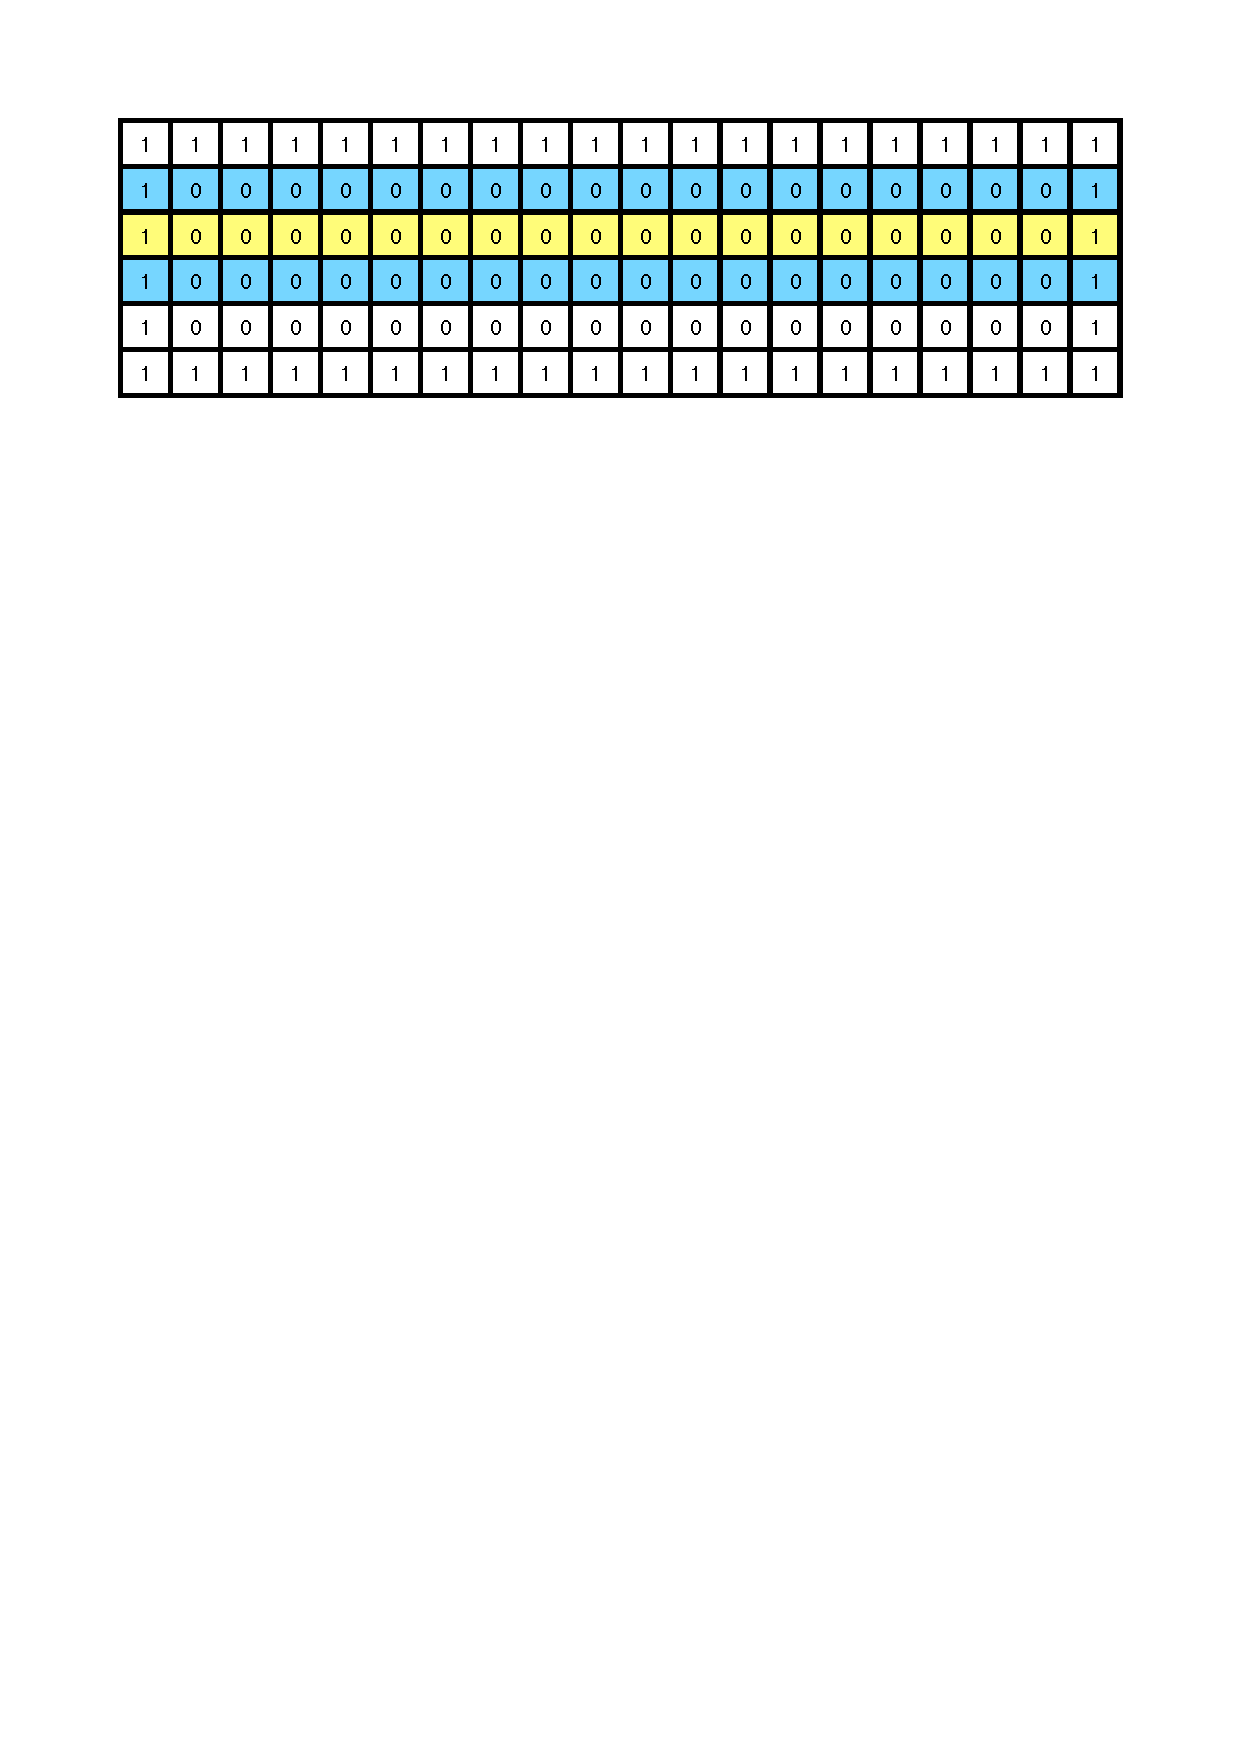
\includegraphics[width=.9\textwidth]{img/rowduplication.pdf}
        \caption{Additional rows required (blue) to relax elements in a single row (yellow).}
        \label{fig:duplicates}
    \end{figure}

As Figure \ref{fig:duplicates} illustrates, irrespective of how many partitions the matrix is split into, each CPU will require the rows immediately before and after its partition in a read-only capacity. This overhead is significant in Figure \ref{fig:duplicates} (200\%), and it can be seen that for an $n\times{n}$ matrix, it is inefficient (i.e. has an overhead $\geq$ 100\%) to have more than $\frac{n-2}{2}$ processors relaxing. From a practical parallelism standpoint, relaxing a matrix with dimensions only double that of the number of available processors is poor exploitation of data parallelism and likely to be slower than a serial equivalent.

The complete $n\times{n}$ matrix is allocated and initialised from the root process and every processor (including the root) allocates space for $2n+\frac{(n-2)(n)}{c} +\frac{(n-2)(n)}{c}$ elements. The additional array of size $+\frac{(n-2)(n)}{c}$ is to preserve the consistency of data being read by performing the \textit{relax} operation; no cell can be overwritten with its new value until the new value every other cell has been calculated. This is the case regardless of whether the relaxation is performed sequentially or in parallel, and necessitates using a second matrix of the same dimensions, into which the relaxed values are written. These dimensions however, do not have to include the $2n$ read-only values from the rows above and below.

This allocation on each of $c$ processors, with an additional $n\times{n}$ on the root, gives a space complexity of $\mathcal{O}(3n^2 -4n + 2nc)$. When calculating space complexity, $c$ is constant as it is simply the number of processors so the space complexity is still asymptotic to $\mathcal{O}(n^2)$; the same space complexity as the shared memory equivalent solution which involved swapping two $n\times{n}$ arrays between iterations.

After each iteration, each process sends the $\frac{n-2}{c}$ rows which it has relaxed back to the root process. In actuality, this is not necessary because only the first and last relaxed rows contain values which are needed by any other process, so only they need to be sent. I decided not to attempt to exploit this because it introduced additional complexity, however if I were attempting to scale my solution to much larger matrices, this would be the first optimisation I would make.

An additional optimisation I could have made was in the calculation of precision. My implementation avoids iterating over cells twice by both relaxing and calculating whether the precision has been reached in the same loop, rather than calculating precision once all cells have been relaxed within a process or from the root process. However, once a process encounters a cell whose new value differs from the old by more than the specified precision, it does not have to calculate the precision for any subsequent cell that iteration. I kept calculating every value however, as some of my testing used small precision values and it was useful that the values of \texttt{local\_continue} and \texttt{global\_continue} were exactly the number of cells where precision had yet to be reached.

\subsection{MPI Strategy}

There are three types of communication which need to happen during the execution of the program, all of them every iteration:
\begin{enumerate}
	\item Sending $2+\frac{n-2}{c}$ rows of the full matrix to each process.\par
			As only a subset of the matrix is required by each process, \texttt{MPI\_Scatter} was the logical solution. However, Scatter requires all chunks to be the same size, which is only the case when $(n-2)$ mod $c=0$. The equivalent for unequal partitions is \texttt{MPI\_Scatterv}, so this is how I send data from the root process at the start of each iteration.
	
	\item Sending $\frac{n-2}{c}$ relaxed rows from each process back to the root. \par
			This communication is essentially symmetric to the previous, so I used \texttt{MPI\_Scatterv}'s counterpart \texttt{MPI\_Gatherv} to communicate the relaxed cells back to the root process.
			
	\item Communication between all processes as to whether another iteration is required.\par
			I considered adding an extra cell to each array sent back to the root process in the previous communication to piggyback the completion status of each processor with its data, but ultimately this seemed an untidy solution to a problem which \texttt{MPI\_Allreduce} could solve. I therefore reduce the \texttt{MPI\_SUM} operation over the values of \texttt{local\_continue} on every processor (where any positive value indicates a cell which has not yet reached the required precision.) If any processor needs to continue, they must all continue.
\end{enumerate}


\section{Correctness Testing}

To verify that my implementation of relaxation was correct, I first manually calculated the first three iterations of the top left corner of the initial matrix from my solution. I then confirmed that my solution generated the same intermediate matrices by running it in verbose mode so it would print the matrix state at the end of every iteration.

\begin{minipage}{.45\textwidth}
$$
\begin{matrix}
1.000000 & 1.000000 & 1.000000 & 1.000000 & \quad\cdots \\
1.000000 & 0.000000 & 0.000000 & 0.000000 & \quad\cdots \\
1.000000 & 0.000000 & 0.000000 & 0.000000 & \quad\cdots \\
1.000000 & 0.000000 & 0.000000 & 0.000000 & \quad\cdots \\
\vdots & \vdots & \vdots & \vdots & \quad\ddots \\
\end{matrix}
$$
$$
\begin{matrix}
1.000000 & 1.000000 & 1.000000 & 1.000000 & \quad\cdots \\
1.000000 & 0.500000 & 0.250000 & 0.250000 & \quad\cdots \\
1.000000 & 0.250000 & 0.000000 & 0.000000 & \quad\cdots \\
1.000000 & 0.250000 & 0.000000 & 0.000000 & \quad\cdots \\
\vdots & \vdots & \vdots & \vdots & \quad\ddots \\
\end{matrix}
$$
$$
\begin{matrix}
1.000000 & 1.000000 & 1.000000 & 1.000000 & \quad\cdots \\
1.000000 & 0.625000 & 0.437500 & 0.375000 & \quad\cdots \\
1.000000 & 0.437500 & 0.125000 & 0.062500 & \quad\cdots \\
1.000000 & 0.375000 & 0.062500 & 0.000000 & \quad\cdots \\
\vdots & \vdots & \vdots & \vdots & \quad\ddots \\
\end{matrix}
$$

\end{minipage}\hspace{2cm}
\begin{minipage}{.42\textwidth}
	To ensure my solution was exhaustively correct, I used one core on each of one to three nodes, relaxing a matrix of dimensions $1000 \times{} 1000$ and precision $p=0.01$, which should require 37 iterations.\\
	
	The output files were too large to manually check, so I used the Unix \texttt{diff} utility to programatically check the similarity of the two and three node runs against the single core on the single node (\texttt{N1-TPN1-batch-1000.out}). The only difference between the output files are the lines which contain job-specific output from SLURM; the actual matrix content is identical.
\end{minipage}

These files are too large to include themselves, so instead I have included the output from \texttt{diff} for two and three nodes against one node, for verification.

\clearpage
\section{Scalability Investigation}

\subsection{Fixed Problem Size}
Once I had verified the correctness of my relaxation implementation, I chose a fixed array size and precision, and ran my program relaxing the same array with 1-64 cores across 1-4 nodes.  The time, speedup and efficiency (speedup achieved by $n$ processors divided by $n$ \citep{speedup}) relative to the serial program can be seen in Figures \ref{fig:time15}, \ref{fig:sp15}, and \ref{fig:eff15}. \footnote{Full data in Appendices \ref{sec:oneNode}, \ref{sec:twoNodes}, \ref{sec:threeNodes}, and  \ref{sec:fourNodes}.}

\begin{figure}[!htbp]
        \centering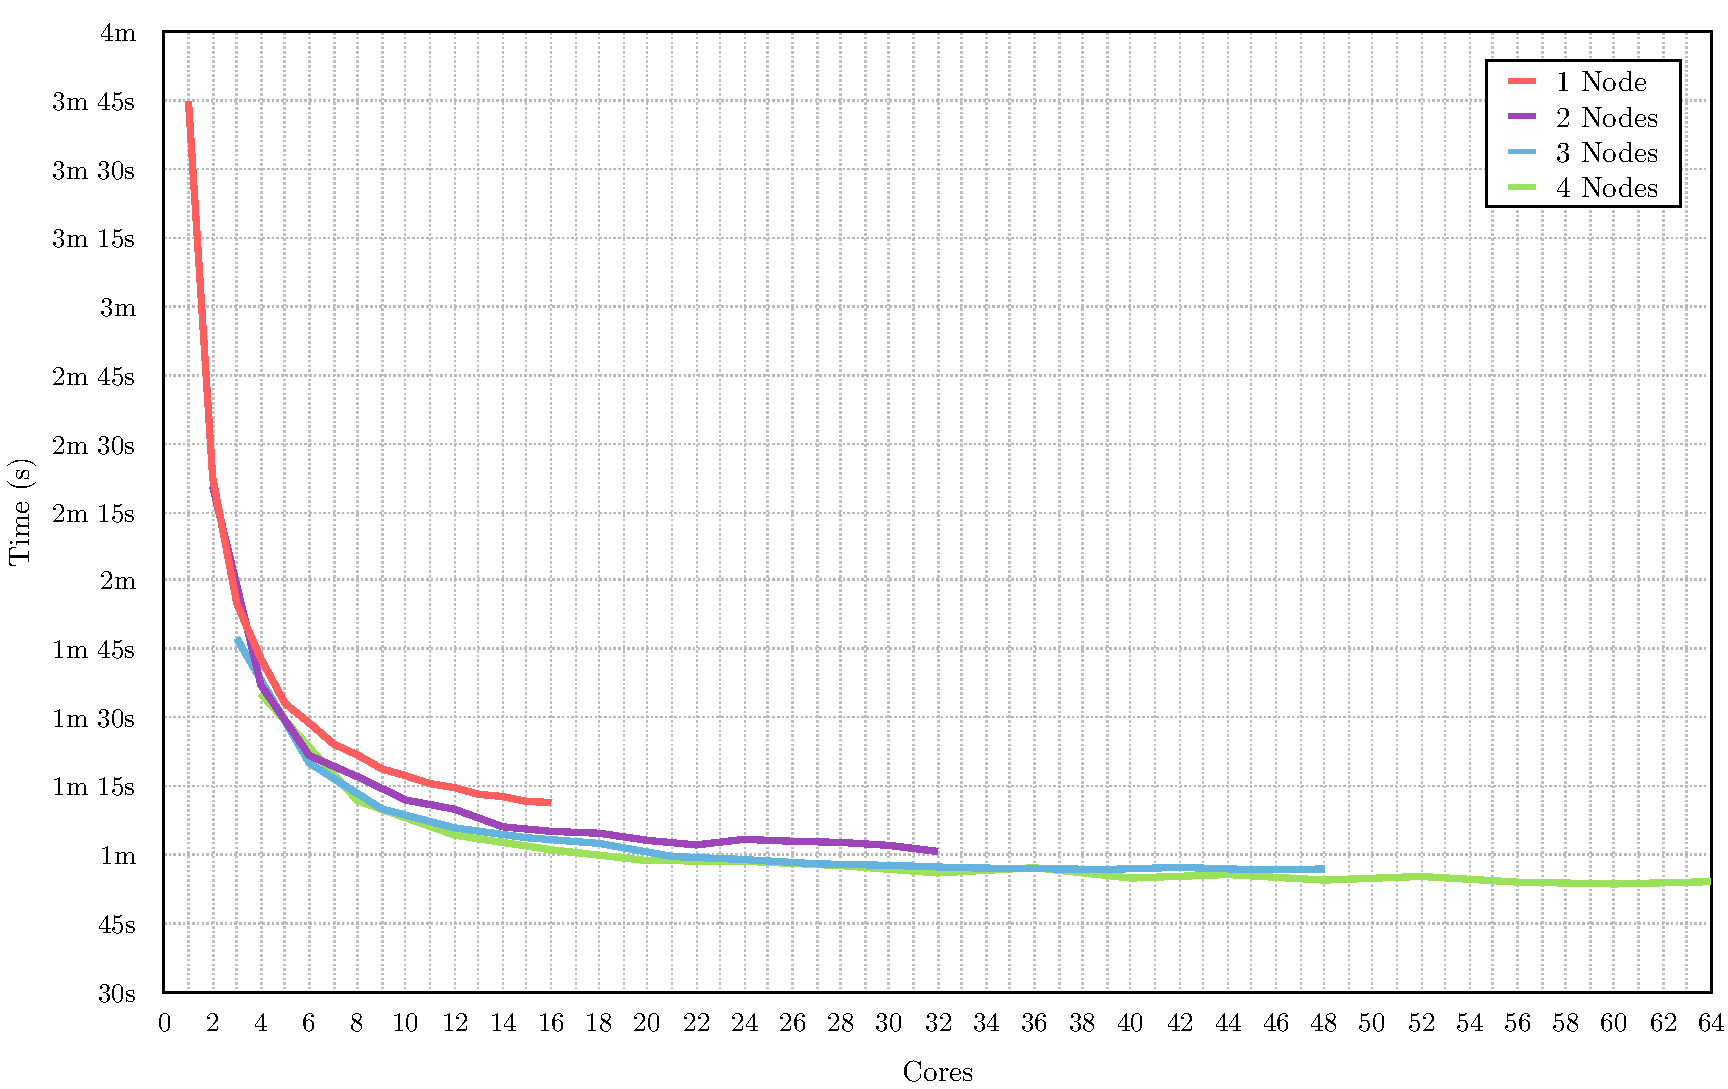
\includegraphics[width=\textwidth]{img/basic-cpus-time.pdf}
        \caption{Time taken for 1-64 cores to relax the same matrix, $d=15000$, $p=0.01$}
        \label{fig:time15}
\end{figure}
\begin{figure}[!htbp]
        \centering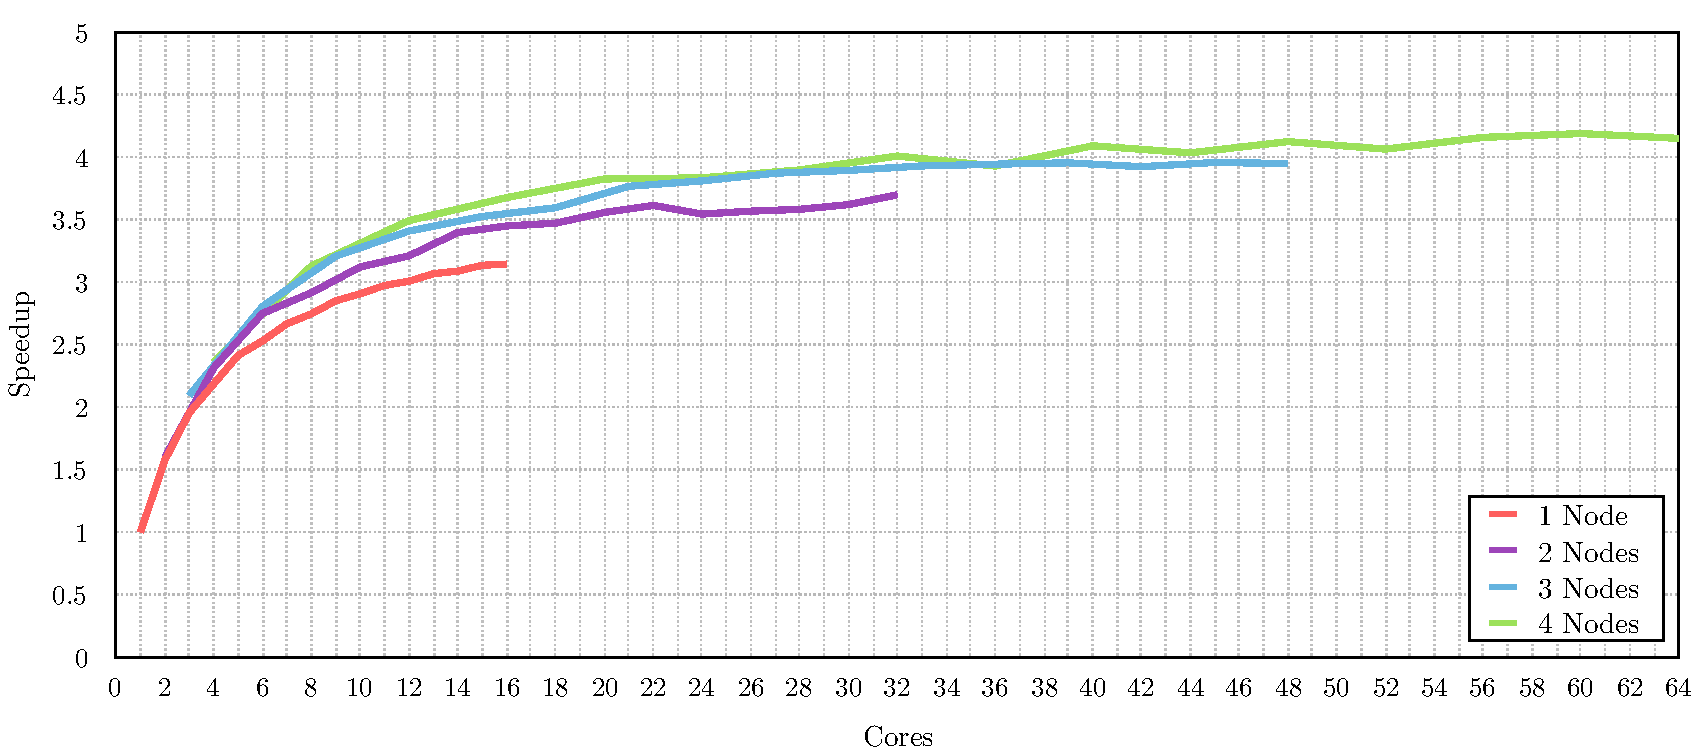
\includegraphics[width=\textwidth]{img/15kspeedup.pdf}
        \caption{Speedup achieved by 1-64 cores relaxing the same matrix, $d=15000$, $p=0.01$}
        \label{fig:sp15}
\end{figure}
\begin{figure}[!htbp]
        \centering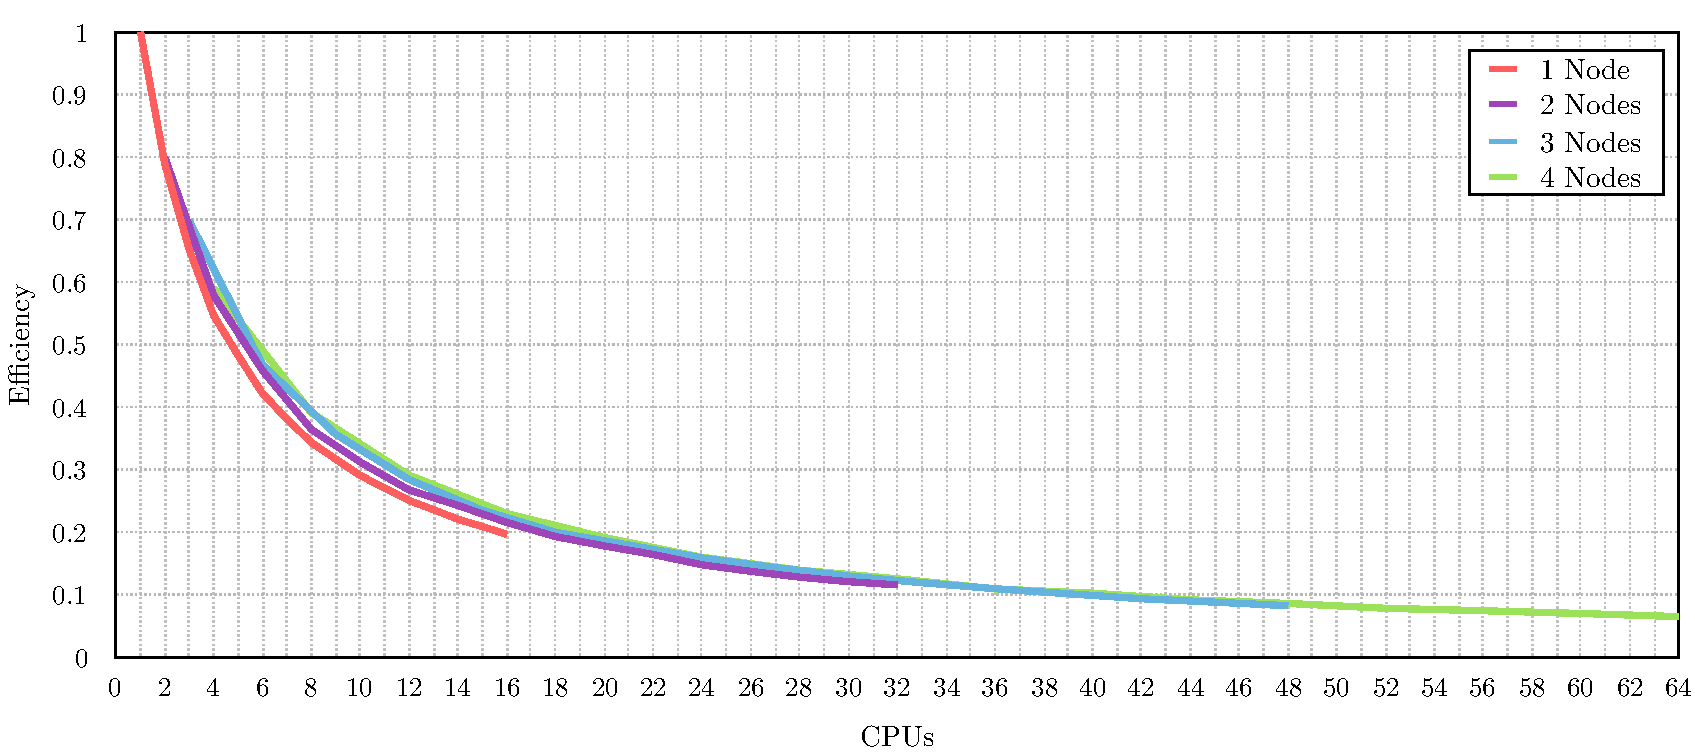
\includegraphics[width=\textwidth]{img/15kefficiency.pdf}
        \caption{Efficiency of 1-64 cores relaxing the same matrix, $d=15000$, $p=0.01$}
        \label{fig:eff15}
\end{figure}

Each additional CPU saw efficiency reduce exponentially, as the speedup had a progressively smaller impact on the time reduction (the principle of diminishing returns; \citep{Amdahl}). This is consistent with Amdahl's law, a corollary of which states that for P processors and a computation whose sequential proportion is denoted $f$, predicted speedup is bound by $\frac{1}{f}$ \citep{springer}. Working backwards from this upper bound and assuming a maximum speedup of 4.2, this would imply that the sequential proportion of my solution is $\leq 0.238$, or 23.8\% of the total computation for this fixed problem size. It is important to note that the sequential proportion is not fixed, as changing the number of cores, precision or dimensions would alter the overhead needed to allocate, assign process work, and wait at barriers.

The speedup I achieved for this problem size was significantly sub-linear in terms of Amdahl's law. The limiting factor is the relatively slow speed of communication between cores, and as the volume of communication necessary increases proportionally to the number of cores, the overhead increases in line with this. The fact that the timing, speedup and efficiency curves are similarly asymptotic for all numbers of nodes suggests that intra-node communication speeds are not as much of a limiting factor as memory access for sensibly large problem sizes.

Also consistent with expectation was the timing and efficiency of different configuratoins for the same number of cores; i.e. one node with 12 cores (1m 14s 745ms, 25.1\% efficiency), two nodes each with six cores (1m 10s 12ms, 26.8\% efficiency), three nodes with four cores (1m 5s 932ms, 28.4\% efficiency), and four nodes with three (1m 4s 357ms, 29.1\% efficiency). Although the absolute difference in timing between the slowest and fastest configuration is under 11 seconds, this translates to a difference in relative efficiencies of 4\%.

These results demonstrate that not only does this problem size achieve diminishing returns when additional cores are added to the total number irrespective of configuration (shown by the exponential decay curve of all four lines in Figure \ref{fig:time15} grouped as one) but also on a cores per node basis for every node (shown by the exponential decay of each individual curve in Figure \ref{fig:cpn}.)
\begin{figure}[htbp!]
        \centering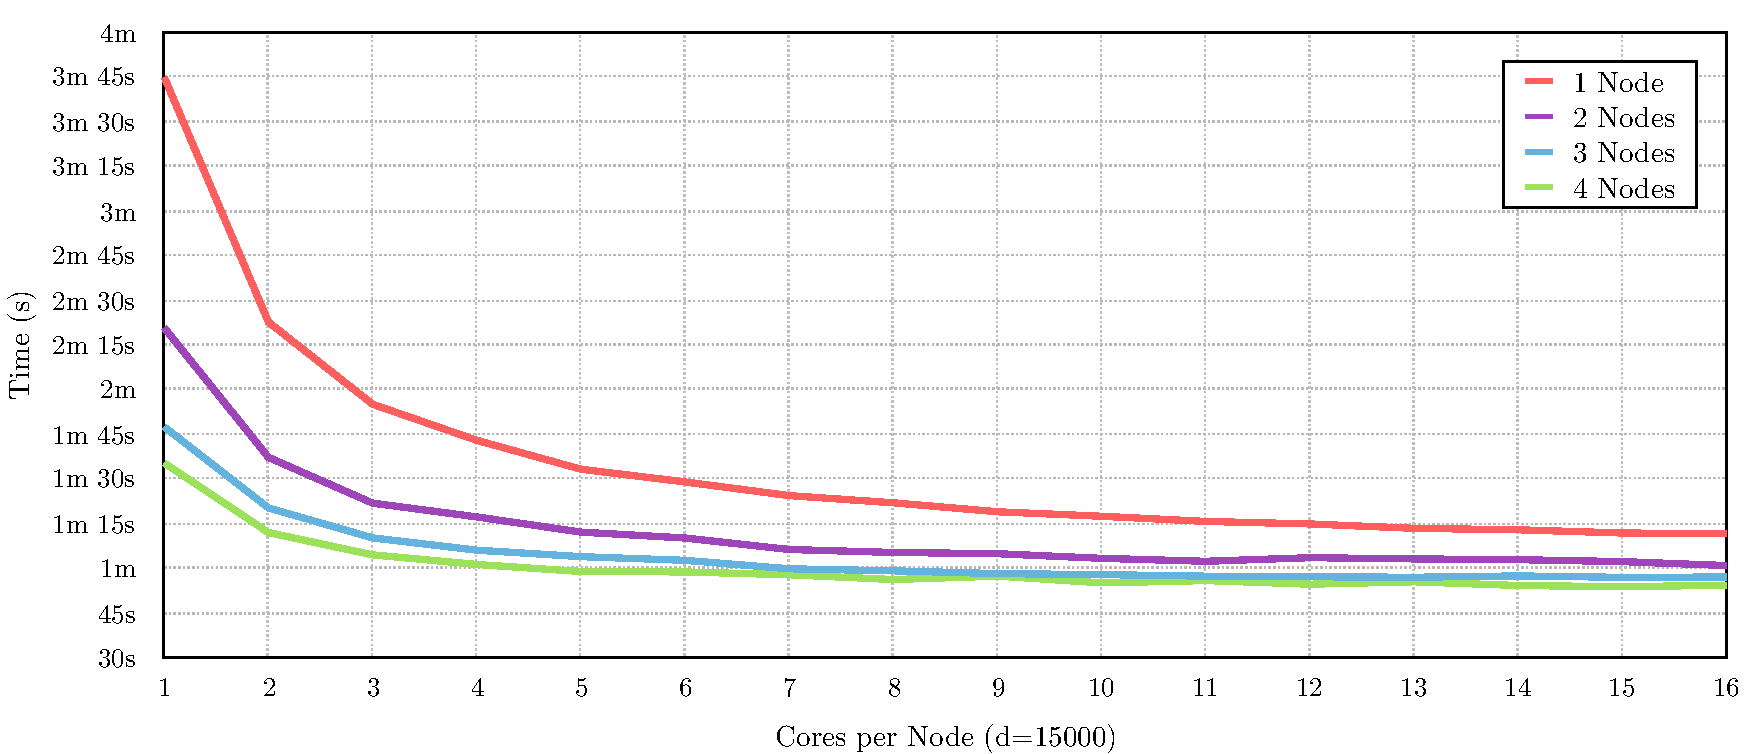
\includegraphics[width=\textwidth]{img/cpn.pdf}
        \caption{Diminishing returns from additional cores per node, $d=15000$, $p=0.01$}
        \label{fig:cpn}
\end{figure}

This difference in configuration speeds is due to the additional memory and bandwidth available to each core when cores are underpopulated on nodes (i.e. not every core is used on each node.) The performance gain from this outweighs the additional communication cost of adding another node for the problem size I initially tested ($15000\times{}15000$), so to confirm that a smaller problem size requiring significantly less memory would not benefit from underpopulated nodes, I ran the same tests on a matrix nine times smaller; $5000\times{}5000$. Figures \ref{fig:time5}, \ref{fig:sp5}, and \ref{fig:eff5} show the results. \footnote{Full data in Appendices \ref{sec:oneNode}, \ref{sec:twoNodes}, \ref{sec:threeNodes}, and  \ref{sec:fourNodes}.}

\begin{figure}[htbp!]
        \centering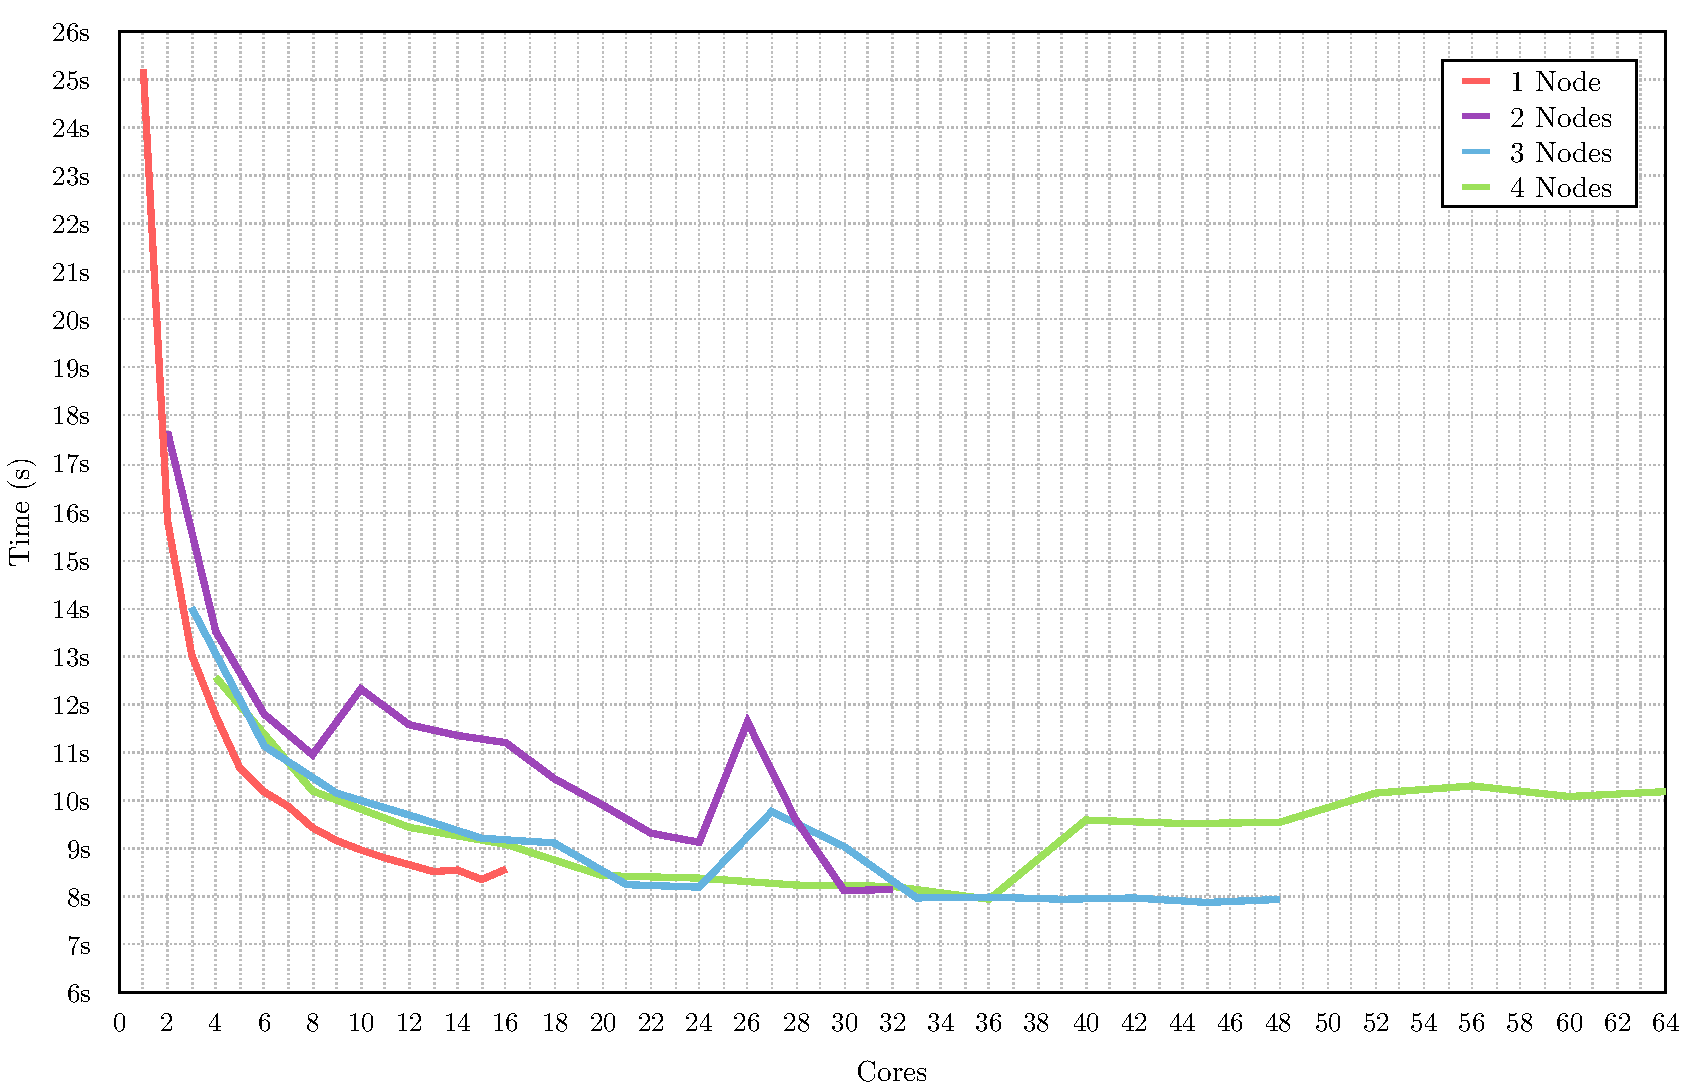
\includegraphics[width=\textwidth]{img/5ktime.pdf}
        \caption{Time taken for 1-64 cores to relax the same matrix, $d=5000$, $p=0.01$}
        \label{fig:time5}
\end{figure}
\begin{figure}[htbp!]
        \centering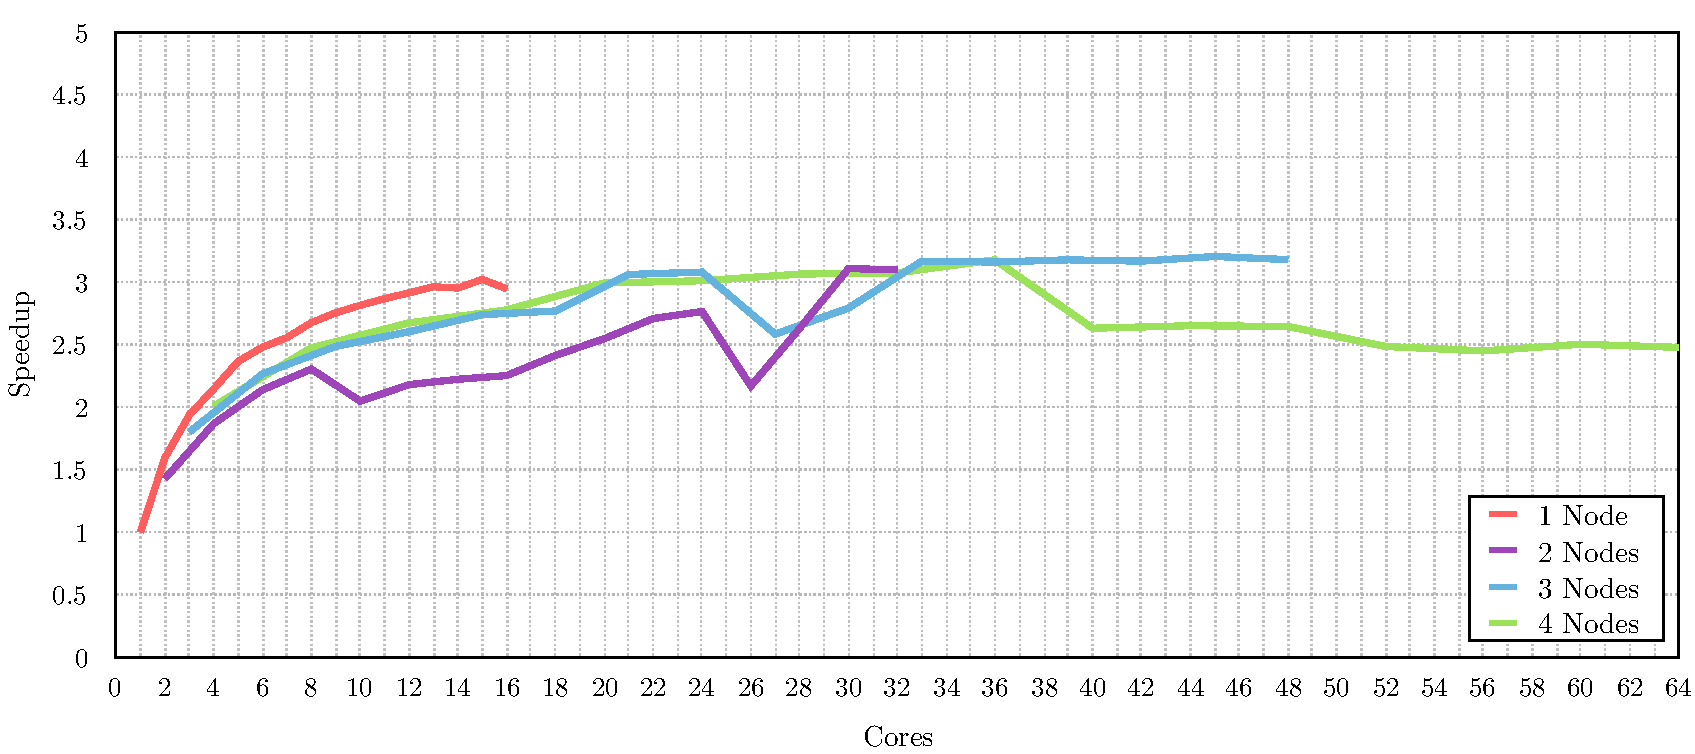
\includegraphics[width=\textwidth]{img/5kspeedup.pdf}
        \caption{Speedup achieved by 1-64 cores relaxing the same matrix, $d=5000$, $p=0.01$}
        \label{fig:sp5}
\end{figure}
\begin{figure}[htbp!]
        \centering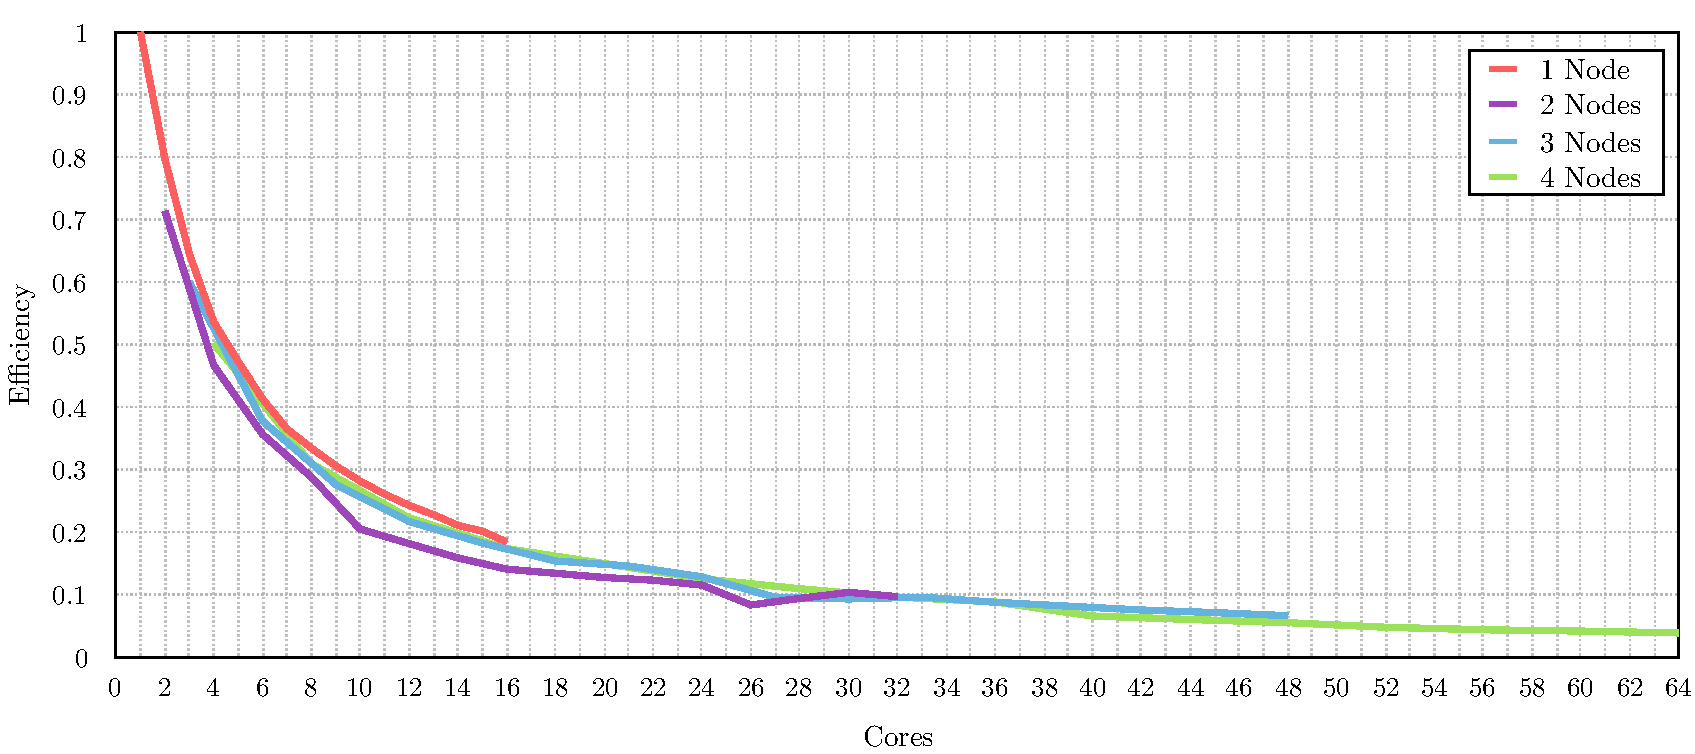
\includegraphics[width=\textwidth]{img/5kefficiency.pdf}
        \caption{Efficiency of 1-64 cores relaxing the same matrix, $d=5000$, $p=0.01$}
        \label{fig:eff5}
\end{figure}

As predicted, with a smaller problem size cores no longer benefit as much from the memory access associated with underpopulated nodes, and because the matrix is smaller but the same number of messages are required, message-passing creates a more significant overhead when using multiple nodes. The one-node-12-core configuration performed best in this case, with the two-node-six-core configuration performing significantly worse than both three and four nodes. For this problem size, the messaging overhead dwarfed the gains of parallelism on four nodes above 36 cores.


\clearpage
\subsection{Variable Problem Size}

The second factor I tested was the effect of varying the matrix dimensions on the time, for various numbers of cores. The results of this can be seen in Figures \ref{fig:dimension-time} and \ref{fig:dimension-sp}. The x-axis in the graph is scaled according to the square of the dimensions tested rather than the dimensions themselves, as the problem size is equal to the number elements of the matrix. \footnote{Full data in Appendices \ref{sec:dtimeout} and \ref{sec:varprob}.}


\begin{figure}[htbp!]
	\centering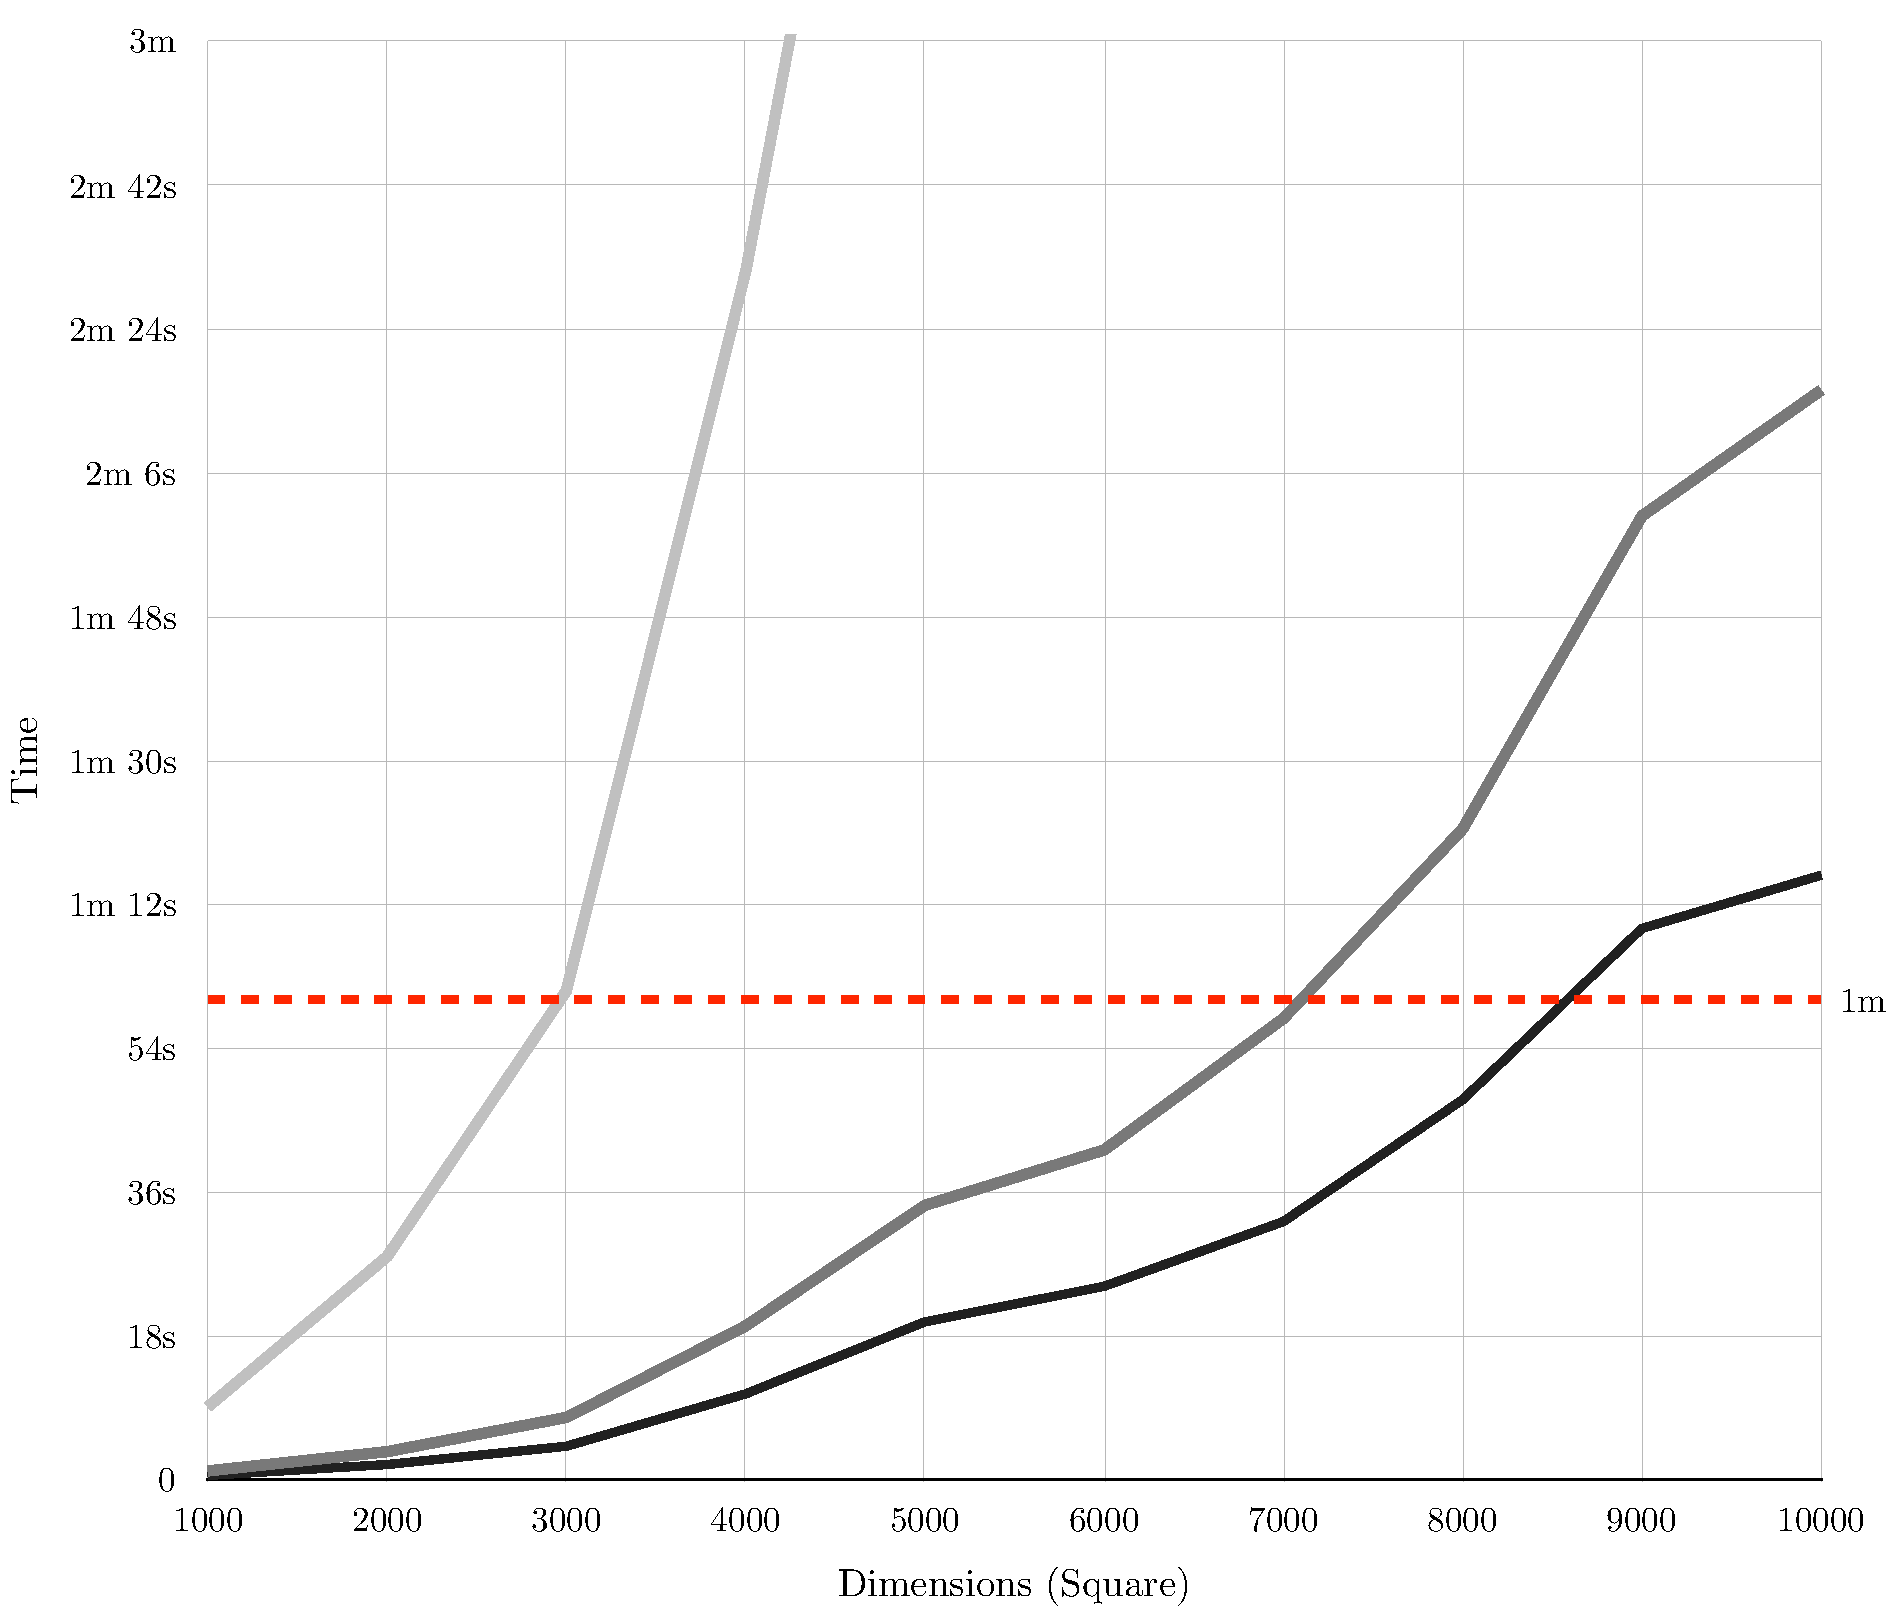
\includegraphics[width=\textwidth]{img/dimension-time.pdf}
	\caption{Matrix size against time for 16, 32, 48 and 64 cores.}
	\label{fig:dimension-time}
\end{figure}

\begin{figure}[htbp!]
	\centering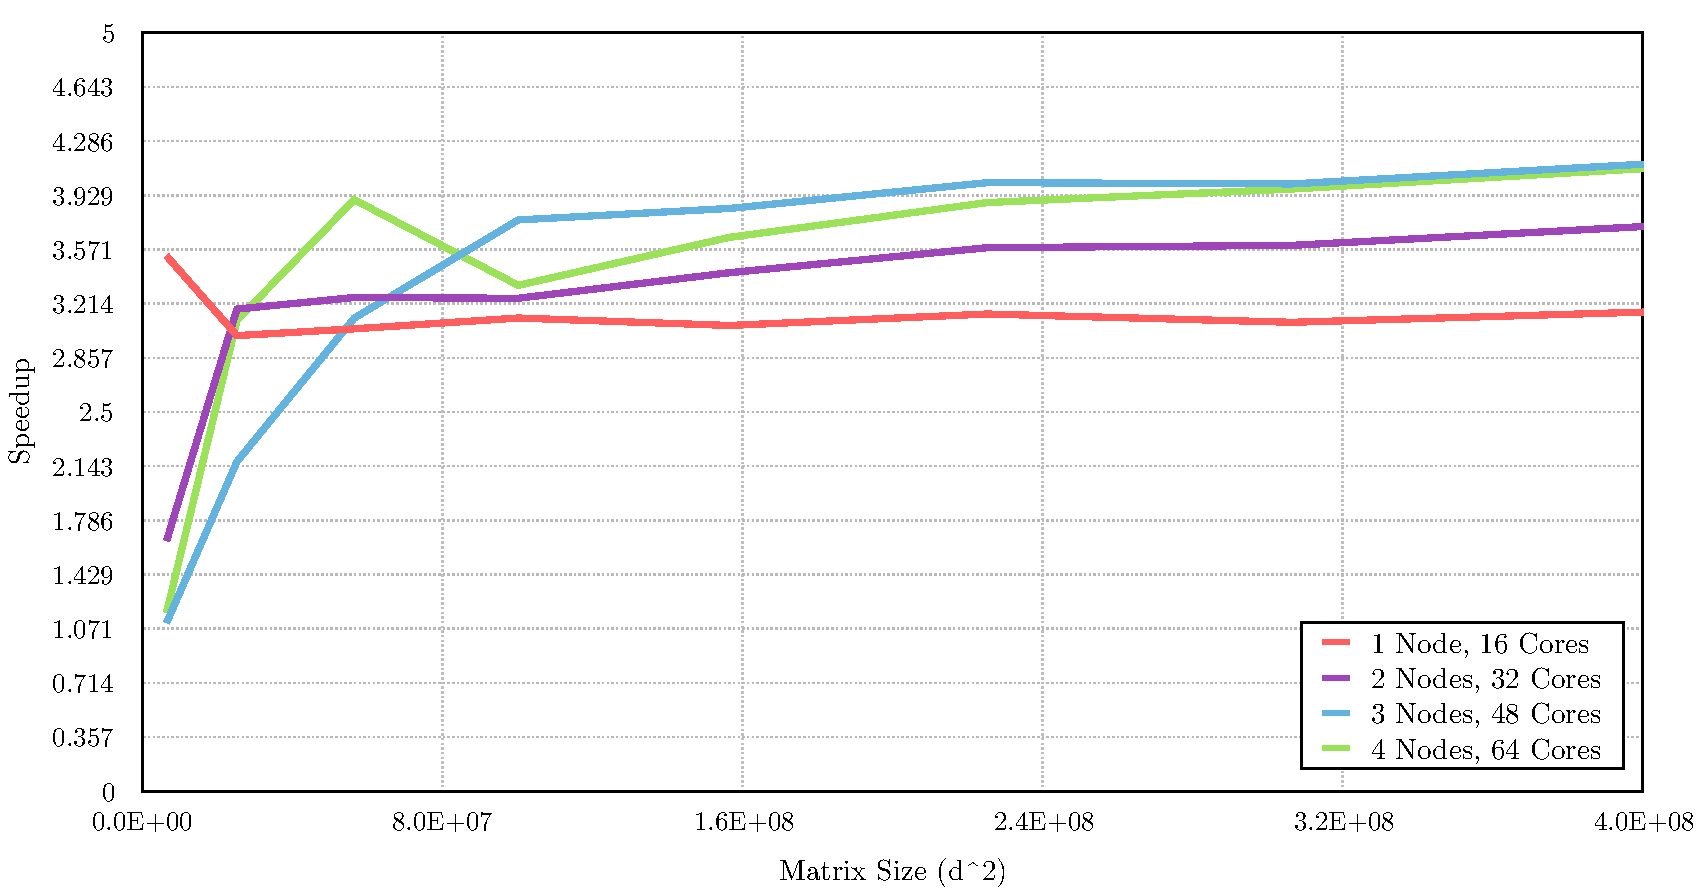
\includegraphics[width=\textwidth]{img/dimension-speedup}
	\caption{Matrix size against speedup for 16, 32, 48 and 64 cores.}
	\label{fig:dimension-sp}
\end{figure}

Time taken increases roughly linearly for a linear increase in matrix size size, as diminishing returns does not apply in the same way to variable problem sizes with fixed computational resources. The maximum matrix dimension my solutions were able to relax was $45000\times{}45000$, after which 32-64 cores exceed the ten minute timeout on Balena. Below 32 cores, the maximum dimensions reached were $42500\times{}42500$.

Figure \ref{fig:dimension-sp} shows the initial speedup achieved up until $20000\times{}20000$, at which point the serial implementation times out and there is nothing against which to benchmark speedup. Initially, 16 cores exhibits the best speedup due to the small problem size; the overhead of sending data off-core to relax dwarfs the relaxation time below $5000\times{}5000$. Above these dimensions, 16 cores settles to a stable speedup of 1.9, with 32 cores seeing an average speedup of 3.4 and 64 cores exhibiting slightly worse speedup than 48 cores above $15000\times{}15000$.

Gustafson's Law argues that as problem size increases, the sequential part of a computation decreases relatively and therefore the speedup achieved by $p$ processors for problem size $n$ is not bound by the sequential proportion $f$ as in Amdahl's law, but $p$ itself (with $S_p = p$ being perfect speedup). However, this law has been shown to be equivalent to Amdahl's law \citep{reevaluating} so I chose not to calculate speedup again.

\clearpage
\subsection{Variable Precision}
I conducted a single experiment into the effects of lowering the precision threshold on the time and iterations required for my solution to terminate. Below are the results for a fixed array with $d=15000$ and varying numbers of cores. The decreased performance of my distributed memory solution for smaller precision values is worse than the performance of my shared version because smaller precisions require many more iterations, and each iteration requires an additional MPI scatter, gather and reduce operation. Therefore, the benefits of parallelism are outweighed by the communication overheads for lower precision values. The exact precision value at which communication becomes the bottleneck is dependant on matrix size, and will decrease as matrix size increases. \footnote{Full data in Appendix \ref{sec:ptimeout}.}

\begin{figure}[htbp!]
	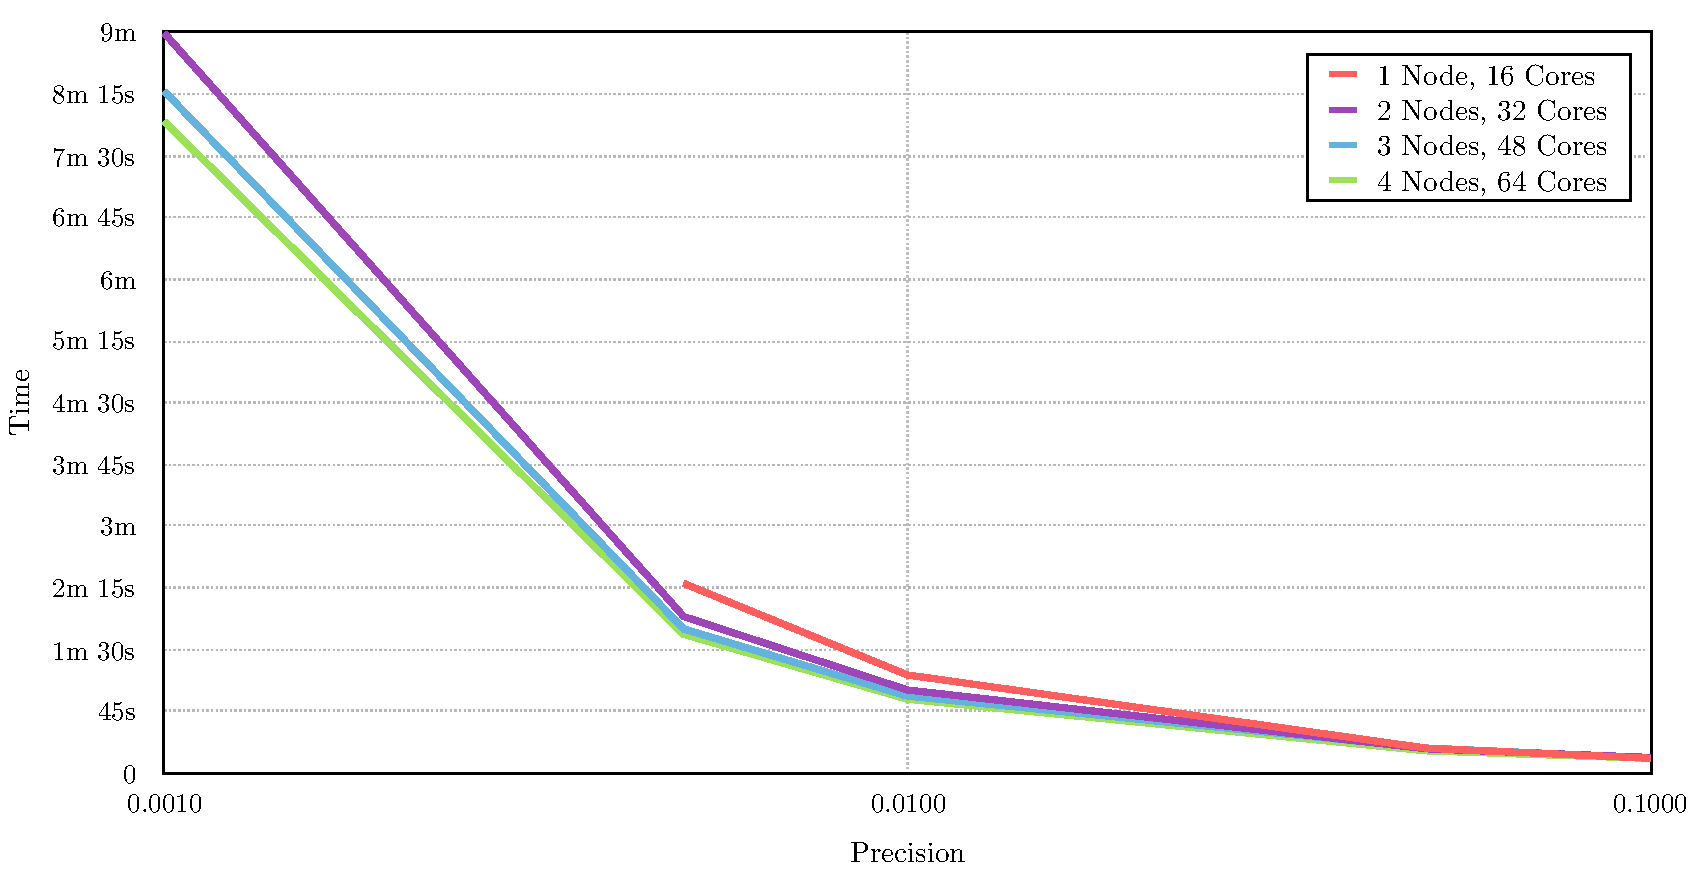
\includegraphics[width=\textwidth]{img/precision.pdf}
	\caption{Time taken relaxing to precision (logarithmic scale), $d=15000$.}
	\label{fig:precision}
\end{figure}

The behaviour my precision tests show is exacerbated by the data I tested it on. A matrix of all 1's on the boundary cells with every other cell initialised to 0 will propagate non-zero values towards the centre of the matrix slowly, and will take the same number of iterations to reach a given precision regardless of size.\footnote{0.1 requires four iterations; 0.01 requires 37 iterations; 0.001 requires 360 iterations.} 
Had I used random doubles in every cell, a larger matrix would typically have taken more iterations and there would not have been as strong a correlation between precision and timing for every matrix.

\clearpage
\bibliography{references}

\begin{appendices}

\clearpage
\section{Full Testing Results}
\vspace{-0.5cm}\subsection{Time, Speedup and Efficiency for 1 Node, 1-16 cores, $p=0.01$}\vspace{-0.5cm}
\footnotesize{\label{sec:oneNode}
\begin{center}
\begin{tabular}{|p{1cm}|p{2.5cm}|p{2cm}|p{2cm}|p{2.5cm}|p{2cm}|p{2cm}|}
\hline
Cores	& Time\par(d=5000)	& Speedup (d=5000)	& Efficiency (d=5000)	& Time \par(d=15000)	& Speedup (d=15000)	& Efficiency (d=15000)  \\
\hline
1	& 25s 219ms	& 1.0000	& 1.0000	& 3m 44s 762ms	& 1.0000	& 1.0000 \\
2	& 15s 817ms	& 1.5944	& 0.7972	& 2m 22s 567ms	& 1.5765	& 0.7883 \\
3	& 13s 24ms	& 1.9363	& 0.6454	& 1m 54s 972ms	& 1.9549	& 0.6516 \\
4	& 11s 752ms	& 2.1459	& 0.5365	& 1m 42s 839ms	& 2.1856	& 0.5464 \\
5	& 10s 660ms	& 2.3658	& 0.4732	& 1m 33s 131ms	& 2.4134	& 0.4827 \\
6	& 10s 171ms	& 2.4795	& 0.4133	& 1m 28s 849ms	& 2.5297	& 0.4216 \\
7	& 9s 866ms	& 2.5562	& 0.3652	& 1m 24s 269ms	& 2.6672	& 0.3810 \\
8	& 9s 425ms	& 2.6758	& 0.3345	& 1m 21s 848ms	& 2.7461	& 0.3433 \\
9	& 9s 155ms	& 2.7547	& 0.3061	& 1m 18s 836ms	& 2.8510	& 0.3168 \\
10	& 8s 961ms	& 2.8143	& 0.2814	& 1m 17s 323ms	& 2.9068	& 0.2907 \\
11	& 8s 793ms	& 2.8681	& 0.2607	& 1m 15s 589ms	& 2.9735	& 0.2703 \\
12	& 8s 655ms	& 2.9138	& 0.2428	& 1m 14s 745ms	& 3.0071	& 0.2506 \\
13	& 8s 511ms	& 2.9631	& 0.2279	& 1m 13s 268ms	& 3.0677	& 0.2360 \\
14	& 8s 542ms	& 2.9524	& 0.2109	& 1m 12s 783ms	& 3.0881	& 0.2206 \\
15	& 8s 345ms	& 3.0220	& 0.2015	& 1m 11s 699ms	& 3.1348	& 0.2090 \\
16	& 8s 560ms	& 2.9461	& 0.1841	& 1m 11s 489ms	& 3.1440	& 0.1965 \\
\hline
\end{tabular}
\end{center}}

\vspace{-0.5cm}\subsection{Time, Speedup and Efficiency for 2 Nodes, 2-32 cores, $p=0.01$}\vspace{-0.5cm}
\footnotesize{\label{sec:twoNodes}
\begin{center}
\begin{tabular}{|p{1cm}|p{2.5cm}|p{2cm}|p{2cm}|p{2.5cm}|p{2cm}|p{2cm}|}
\hline
Cores	& Time\par(d=5000)	& Speedup (d=5000)	& Efficiency (d=5000)	& Time \par(d=15000)	& Speedup (d=15000)	& Efficiency (d=15000)  \\
\hline
2 & 17s 672ms & 1.4271 & 0.7135 & 2m 20s 616ms & 1.5984 & 0.7992 \\
4 & 13s 506ms & 1.8672 & 0.4668 & 1m 37s 111ms & 2.3145 & 0.5786 \\
6 & 11s 791ms & 2.1388 & 0.3565 & 1m 21s 733ms & 2.7500 & 0.4583 \\
8 & 10s 944ms & 2.3044 & 0.2880 & 1m 17s 103ms & 2.9151 & 0.3644 \\
10 & 12s 315ms & 2.0478 & 0.2048 & 1m 12s 6ms & 3.1214 & 0.3121 \\
12 & 11s 569ms & 2.1799 & 0.1817 & 1m 10s 12ms & 3.2103 & 0.2675 \\
14 & 11s 346ms & 2.2227 & 0.1588 & 1m 6s 158ms & 3.3974 & 0.2427 \\
16 & 11s 196ms & 2.2525 & 0.1408 & 1m 5s 165ms & 3.4491 & 0.2156 \\
18 & 10s 447ms & 2.4140 & 0.1341 & 1m 4s 749ms & 3.4713 & 0.1928 \\
20 & 9s 899ms & 2.5476 & 0.1274 & 1m 3s 186ms & 3.5571 & 0.1779 \\
22 & 9s 311ms & 2.7085 & 0.1231 & 1m 2s 197ms & 3.6137 & 0.1643 \\
24 & 9s 120ms & 2.7652 & 0.1152 & 1m 3s 414ms & 3.5444 & 0.1477 \\
26 & 11s 630ms & 2.1684 & 0.0834 & 1m 2s 998ms & 3.5678 & 0.1372 \\
28 & 9s 588ms & 2.6303 & 0.0939 & 1m 2s 742ms & 3.5823 & 0.1279 \\
30 & 8s 113ms & 3.1085 & 0.1036 & 1m 2s 88ms & 3.6201 & 0.1207 \\
32 & 8s 140ms & 3.0982 & 0.0968 & 1m 0s 763ms & 3.6990 & 0.1156 \\
\hline
\end{tabular}
\end{center}}

\vspace{-0.5cm}\subsection{Time, Speedup and Efficiency for 3 Nodes, 3-48 cores, $p=0.01$}\vspace{-0.5cm}
\footnotesize{\label{sec:threeNodes}
\begin{center}
\begin{tabular}{|p{1cm}|p{2.5cm}|p{2cm}|p{2cm}|p{2.5cm}|p{2cm}|p{2cm}|}
\hline
Cores	& Time\par(d=5000)	& Speedup (d=5000)	& Efficiency (d=5000)	& Time \par(d=15000)	& Speedup (d=15000)	& Efficiency (d=15000)  \\
\hline
3 & 14s 5ms &	1.8007 &	0.6002 & 1m 47s 343ms &	2.0939 & 0.6980 \\
6 & 11s 128ms &	2.2663 &	0.3777 & 1m 20s 113ms &	2.8056 & 0.4676 \\
9 & 10s 143ms &	2.4863 &	0.2763 & 1m 10s 61ms &	3.2081 & 0.3565 \\
12 & 9s 688ms &	2.6031 &	0.2169 & 1m 5s 932ms &	3.4090 & 0.2841 \\
15 & 9s 205ms &	2.7397 &	0.1826 & 1m 3s 764ms &	3.5249 & 0.2350 \\
18 & 9s 107ms &	2.7692 &	0.1538 & 1m 2s 520ms &	3.5950 & 0.1997 \\
21 & 8s 238ms &	3.0613 &	0.1458 & 59s 677ms &	3.7663 & 0.1793 \\
24 & 8s 187ms &	3.0804 &	0.1283 & 58s 995ms &	3.8098 & 0.1587 \\
27 & 9s 759ms &	2.5842 &	0.0957 & 58s 57ms &	3.8714 & 0.1434 \\
30 & 9s 32ms &	2.7922 &	0.0931 & 57s 725ms &	3.8937 & 0.1298 \\
33 & 7s 962ms &	3.1674 &	0.0960 & 57s 201ms &	3.9293 & 0.1191 \\
36 & 7s 979ms &	3.1607 &	0.0878 & 56s 996ms &	3.9435 & 0.1095 \\
39 & 7s 935ms &	3.1782 &	0.0815 & 56s 839ms &	3.9544 & 0.1014 \\
42 & 7s 961ms &	3.1678 &	0.0754 & 57s 288ms &	3.9234 & 0.0934 \\
45 & 7s 868ms &	3.2053 &	0.0712 & 56s 800ms &	3.9571 & 0.0879 \\
48 & 7s 931ms &	3.1798 &	0.0662 & 56s 917ms &	3.9489 & 0.0823 \\
\hline
\end{tabular}
\end{center}}

\vspace{-0.5cm}\subsection{Time, Speedup and Efficiency for 4 Nodes, 4-64 cores, $p=0.01$}\vspace{-0.5cm}
\footnotesize{\label{sec:fourNodes}
\begin{center}
\begin{tabular}{|p{1cm}|p{2.5cm}|p{2cm}|p{2cm}|p{2.5cm}|p{2cm}|p{2cm}|}
\hline
Cores	& Time\par(d=5000)	& Speedup (d=5000)	& Efficiency (d=5000)	& Time \par(d=15000)	& Speedup (d=15000)	& Efficiency (d=15000)  \\
\hline
4 &	12s 558ms &	2.0082	 & 0.5021 & 1m 35s 199ms &	2.3610	 & 0.5902 \\
8 &	10s 191ms &	2.4746	 & 0.3093 & 1m 11s 843ms &	3.1285	 & 0.3911 \\
12 &	9s 432ms &	2.6738	 & 0.2228 & 1m 4s 357ms &	3.4924	 & 0.2910 \\
16 &	9s 78ms &	2.7780	 & 0.1736 & 1m 1s 139ms &	3.6762	 & 0.2298 \\
20 &	8s 426ms &	2.9930	 & 0.1496 & 58s 757ms &	3.8253	 & 0.1913 \\
24 &	8s 375ms &	3.0112	 & 0.1255 & 58s 621ms &	3.8342	 & 0.1598 \\
28 &	8s 230ms &	3.0643	 & 0.1094 & 57s 669ms &	3.8974	 & 0.1392 \\
32 &	8s 203ms &	3.0744	 & 0.0961 & 56s 67ms &	4.0088	 & 0.1253 \\
36 &	7s 934ms &	3.1786	 & 0.0883 & 57s 213ms &	3.9285	 & 0.1091 \\
40 &	9s 585ms &	2.6311	 & 0.0658 & 54s 948ms &	4.0904	 & 0.1023 \\
44 &	9s 512ms &	2.6513	 & 0.0603 & 55s 715ms &	4.0341	 & 0.0917 \\
48 &	9s 534ms &	2.6452	 & 0.0551 & 54s 502ms &	4.1239	 & 0.0859 \\
52 &	10s 147ms &	2.4854	 & 0.0478 & 55s 304ms &	4.0641	 & 0.0782 \\
56 &	10s 295ms &	2.4496	 & 0.0437 & 54s 57ms &	4.1579	 & 0.0742 \\
60 &	10s 75ms &	2.5031	 & 0.0417 & 53s 661ms &	4.1886	 & 0.0698 \\
64 &	10s 177ms &	2.4780	 & 0.0387 & 54s 159ms &	4.1500	 & 0.0648 \\
\hline
\end{tabular}
\end{center}}

\vspace{-0.5cm}\subsection{Increasing $d$ until timeout for 1-64 cores, $p=0.01$}\vspace{-0.5cm}
\footnotesize{\label{sec:dtimeout}
\begin{center}
\begin{tabular}{|p{1cm}|p{2cm}|p{2.2cm}|p{2.2cm}|p{2.2cm}|p{2.2cm}|p{2.2cm}|}
\hline
$d$ & Problem Size\par (Elements) & 1 Core \par(1 Node) & 16 Cores \par(1 Node) & 32 Cores \par(2 Nodes) & 48 Cores \par(3 Nodes) & 64 Cores \par(4 Nodes) \\
\hline
2500 & 6250000 & 6s 552ms & 	1s 859ms & 	3s 974ms & 	5s 911ms & 	5s 567ms \\
5000 & 25000000 & 25s 234ms & 	8s 412ms & 	7s 949ms & 	11s 629ms & 	8s 142ms  \\ 
7500 & 56250000 & 56s 154ms & 	18s 444ms & 	17s 274ms & 	18s 28ms & 	14s 416ms  \\ 
10000 & 100000000 & 1m 39s 576ms & 	31s 959ms & 	30s 678ms & 	26s 471ms & 	29s 895ms  \\ 
12500 & 156250000 & 2m 35s 101ms & 	50s 576ms & 	45s 430ms & 	40s 419ms & 	42s 529ms  \\ 
15000 & 225000000 & 3m 44s 801ms & 	1m 11s 543ms & 	1m 2s 813ms & 	56s 98ms & 	57s 996ms  \\ 
17500 & 306250000 & 5m 4s 816ms & 	1m 38s 726ms & 	1m 24s 808ms & 	1m 16s 225ms & 	1m 16s 873ms  \\ 
20000 & 400000000 & 6m 39s 895ms & 	2m 6s 760ms & 	1m 47s 544ms & 	1m 36s 847ms & 	1m 37s 549ms  \\ 
22500 & 506250000 & Timeout &	2m 42s 738ms & 	2m 15s 975ms & 	2m 5s 643ms & 	1m 58s 543ms  \\ 
25000 & 625000000 & Timeout &	3m 18s 213ms & 	2m 44s 362ms & 	2m 31s 978ms & 	2m 25s 799ms  \\ 
27500 & 756250000 & Timeout &	4m 3s 95ms & 	3m 18s 385ms & 	3m 5s 9ms & 	2m 57s 622ms  \\ 
30000 & 900000000 & Timeout &	4m 44s 190ms & 	3m 52s 550ms & 	3m 37s 376ms & 	3m 27s 204ms  \\ 
32500 & 1056250000 & Timeout &	5m 38s 698ms & 	4m 36s 622ms & 	4m 15s 270ms & 	4m 6s 17ms  \\ 
35000 & 1225000000 & Timeout &	6m 26s 794ms & 	5m 19s 397ms & 	4m 51s 592ms & 	4m 41s 424ms \\ 
37500 & 1406250000 & Timeout &	7m 31s 775ms & 	6m 7s 474ms & 	5m 39s 128ms & 	5m 24s 8ms  \\ 
40000 & 1600000000 & Timeout &	8m 25s 86ms & 	6m 52s 615ms & 	6m 18s 391ms & 	6m 3s 799ms  \\ 
42500 & 1806250000 & Timeout &	10m 7s 186ms & 	7m 51s 536ms & 	7m 14s 315ms & 	6m 57s 435ms  \\ 
45000 & 2025000000 & Timeout &	Timeout &	8m 39s 503ms & 	8m 1s 642ms & 	7m 41s 298ms \\
47500 & 2256250000 & Timeout &	Timeout &	Timeout &	Timeout &	Timeout \\
\hline
\end{tabular}
\end{center}}

\clearpage
\subsection{Speedup and Efficiency for variable problem size on 1-64 cores until serial timeout, $p=0.01$}\vspace{-0.5cm}
\footnotesize{\label{sec:varprob}
\begin{center}
\begin{tabular}{|p{0.8cm}|p{1.6cm}|p{1.6cm}|p{1.6cm}|p{1.6cm}|p{1.6cm}|p{1.6cm}|p{1.6cm}|p{1.6cm}|p{1.6cm}|}
\hline
$d$ & Speedup (16 Cores) & Efficiency (16 Cores) & Speedup (32 Cores) & Efficiency (32 Cores) & Speedup (48 Cores) & Efficiency (48 Cores) & Speedup (64 Cores) & Efficiency (64 Cores) \\
\hline
2500 & 3.52448 & 0.22028 & 1.64872 & 0.05152 & 1.10844 & 0.02309 & 1.1769 & 0.0184 \\
5000 & 2.99976 & 0.18749 & 3.17449 & 0.09920 & 2.16992 & 0.04521 & 3.0992 & 0.0484 \\
7500 & 3.04457 & 0.19029 & 3.25078 & 0.10159 & 3.11482 & 0.06489 & 3.8953 & 0.0609 \\
10000 & 3.11574 & 0.19473 & 3.24584 & 0.10143 & 3.76170 & 0.07837 & 3.3309 & 0.0520 \\
12500 & 3.06669 & 0.19167 & 3.41407 & 0.10669 & 3.83733 & 0.07994 & 3.6469 & 0.0570 \\
15000 & 3.14218 & 0.19639 & 3.57889 & 0.11184 & 4.00729 & 0.08349 & 3.8761 & 0.0606 \\
17500 & 3.08749 & 0.19297 & 3.59419 & 0.11232 & 3.99890 & 0.08331 & 3.9652 & 0.0620 \\
20000 & 3.15474 & 0.19717 & 3.71843 & 0.11620 & 4.12914 & 0.08602 & 4.0994 & 0.0641 \\
\hline
\end{tabular}
\end{center}}

\subsection{Decreasing $p$ until timeout for 16-64 cores, $d=15000$}\vspace{-0.5cm}
\footnotesize{\label{sec:ptimeout}
\begin{center}
\begin{tabular}{|p{2.5cm}|p{2.5cm}|p{2.5cm}|p{2.5cm}|p{2.5cm}|p{2.5cm}|}
\hline
$p$ & Iterations & 16 Cores (1 Node) & 32 Cores (2 Nodes) & 48 Cores (3 Nodes) & 64 Cores (4 Nodes)\\
\hline
0.100000 & 4 & 10s 812ms &	11s 410ms &	11s 37ms &	10s 755ms \\
0.050000 & 8 & 18s 145ms &	17s 718ms &	18s 273ms &	16s 231ms \\
0.010000 & 37 & 1m 11s 543ms &	1m 0s 581ms &	56s 133ms &	53s 876ms \\
0.005000 & 73 & 2m 18s 259ms &	1m 54s 97ms &	1m 45s 55ms &	1m 41s 139ms \\
0.001000 & 360 & Timeout & 8m 59s 277ms &	8m 16s 915ms &	7m 55s 18ms \\
\hline
\end{tabular}
\end{center}}

	
\end{appendices}

\end{document}